\label{chap:dot_d}
\paragraph{}
One of the two algorithms we implemented for matrix multiplication was what we call the dot\_d algorithm. This algorithm takes full advantage of the flexibility of the annotations, and is capable of using inputs which are distributed across, among other things, arbitrary numbers of localities, and non-uniform (but still rectangular) tiling schemes. This is in contrast to the requirements of Cannon's algorithm, which requires a perfect square number of participating localities and a uniform tiling.
\paragraph{}
This algorithm uses the local tile of the LHS operand to set the pace for the computations it performs. What this means is that the LHS operand defines many aspects of the computation rather than depending on information about both the LHS and RHS. For one thing, the algorithm requests only portions of other tiles which overlap in a relevant way with the local LHS data. This could mean, for example, that some computational node X does not even make use of the entirety of the local RHS tile on X. It allows some other LHS residing on node Y which needs the data to request the leftovers of the RHS on X, rather than node X requesting the data missing from its own LHS  from some other node Z, in order to take full advantage of X's local RHS data. Figure \ref{Fig_7} displays this situation. Although most algorithms do not have this sort of flexibility as a requirement, as mentioned previously it pairs nicely with the very restrictive Cannon's algorithm for supplying options to users, or the tiling optimizer.
\paragraph{}
The dot\_d primitive uses the annotations directly in the multiplication step by iterating through all tiles in the RHS, searching for those which have a relevant overlap, and calculating the submatrix result in its output matrix. In the process of matrix multiplication, when multiplying two matrices $A=B\cdot C$, with $B \in M_{\alpha \times \beta}$, and $C \in M_{\beta \times \kappa}$, we perform $\alpha \times \kappa$ total dot products (row of LHS times column of RHS). When we are performing tile multiplication, we are multiplying a subset of one matrix by a subset of another. We can represent this as tiles $$B_i, B_i \in M_{\alpha_i \times \beta_i}, \sum_{i}^{} \alpha_{B,i} = \alpha$$ $$C_i, C_i \in M_{\beta_i \times \kappa_i}, \sum_{i}^{} \kappa_{C,i} = \kappa$$ $$\sum_{i}^{} \beta_{B, i} = \sum_{i}^{} \beta_{C, i} = \beta$$

\paragraph{}
In order to compute the result matrix $A$, one node in the dot\_d execution holds one $B_i$, its local LHS tile, as well as one $C_i$ its local RHS tile. It iterates through all of the known $C_j$, searching for any tile which has any range of rows which is a subset of the range of columns which $B_i$ posesses. When it has found one, it takes the subset of $B_i$ which has the same range of columns as the range of rows which the $C_j$ has, and stores their product as part of the output tile $A_i$. The dot\_d primitive generates output tiles with dimensions of the number of rows in $B_i$ by the number of columns in $C_i$. It is worth noting that although we have been referring to dot\_d as an algorithm which can tolerate arbitrary tilings, it is required that the tiles of $B$ form a tile row with homogeneous boundaries. That is, if one tile has rows $[25,50)$, and another tile has rows $[24,49)$, these boundaries are nonhomogeneous, and will cause an error. The same is true of $C$, albeit with respect to tile columns. Figure \ref{Fig_6} demonstrates these aspects of the tile output size, and its relation to the tile input size.

\begin{figure}
	\centering
	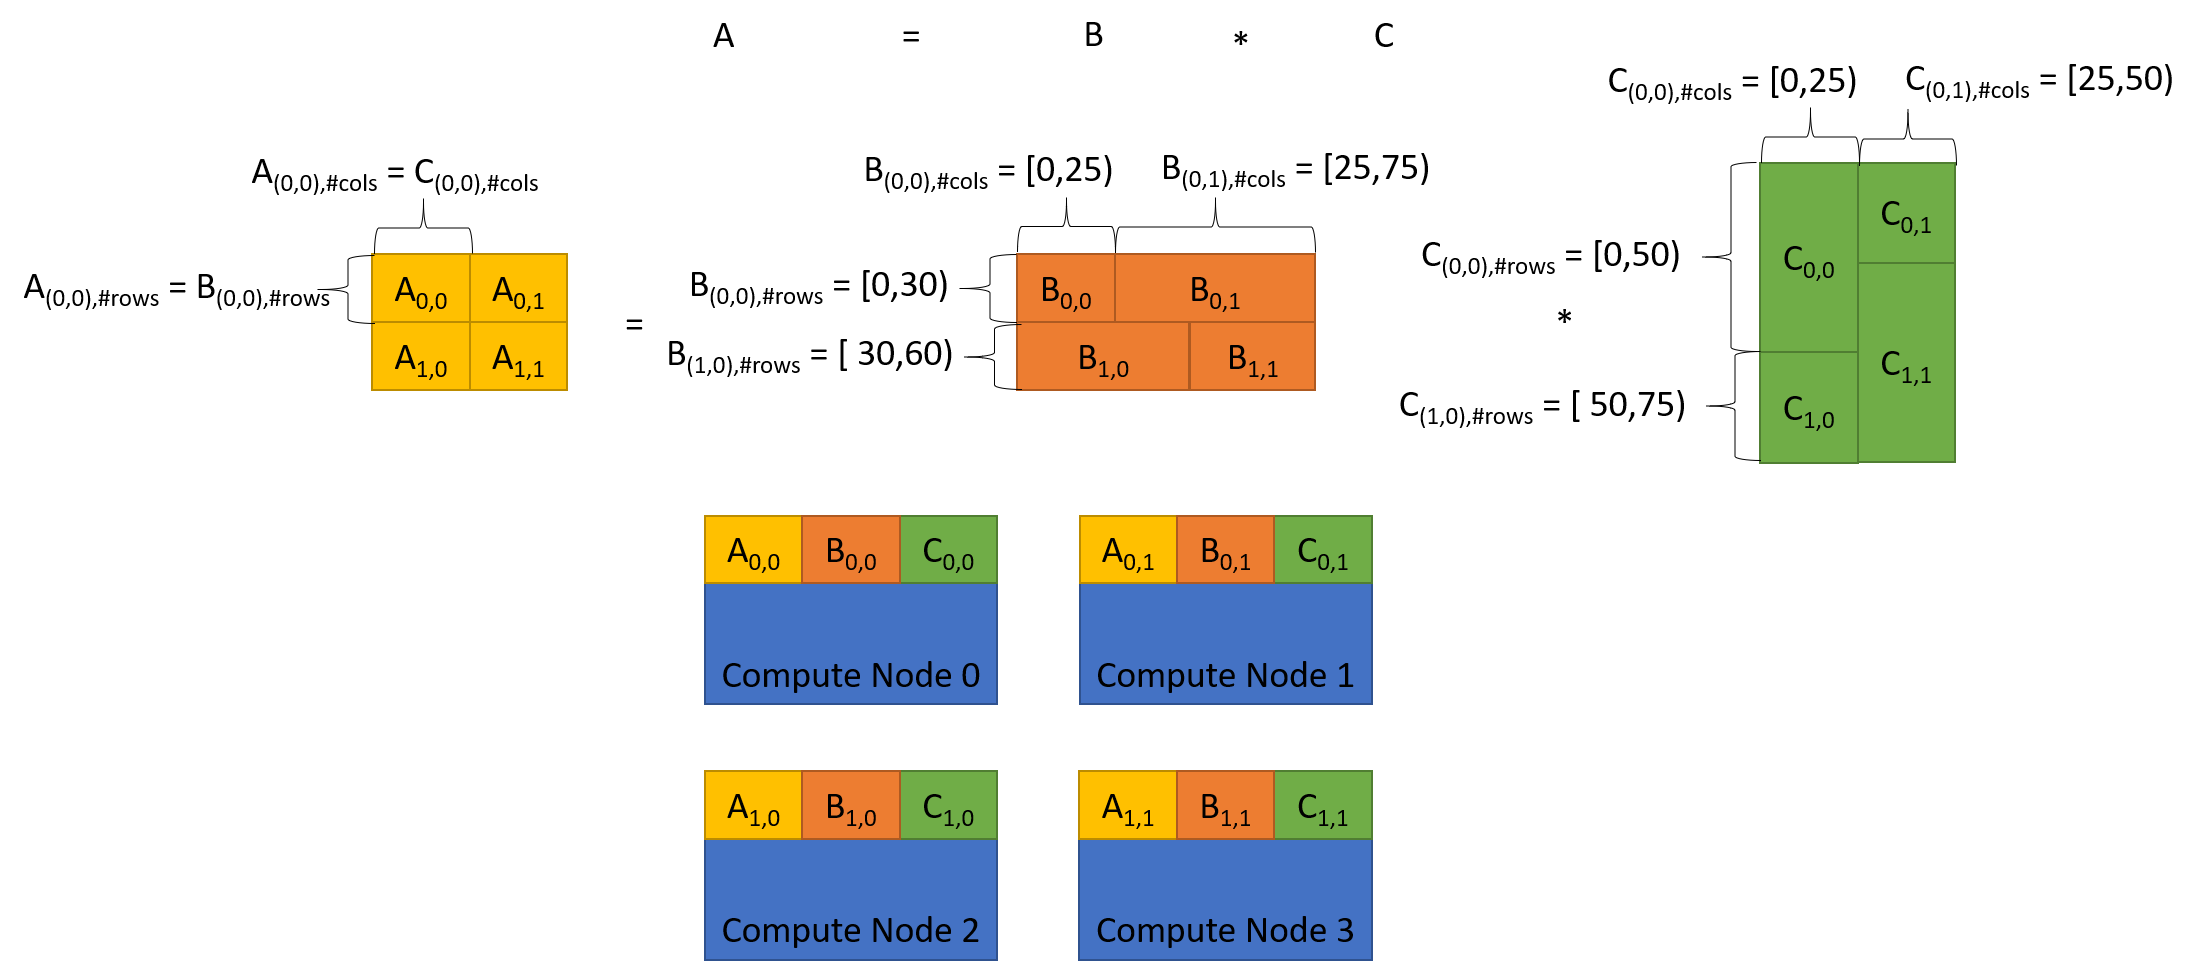
\includegraphics[width=170mm]{calculating_tile_output_size}
	\caption{Calculating Tile Output Size}
	\label{Fig_6}
\end{figure}

\begin{figure}
	\centering
	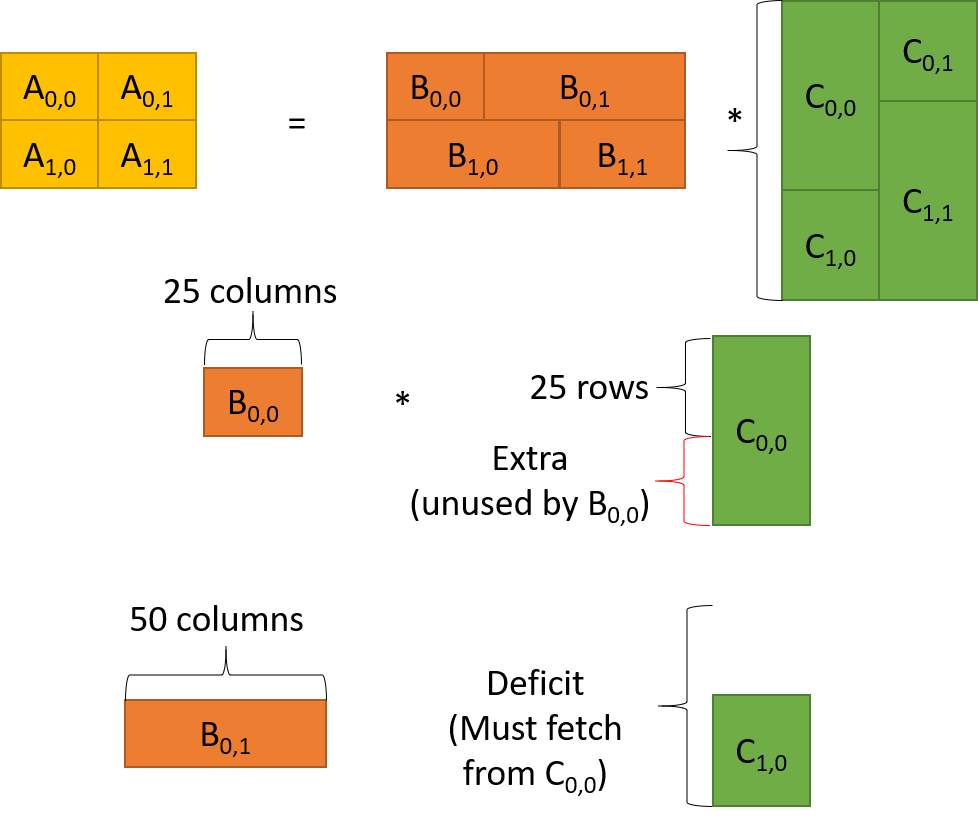
\includegraphics[width=100mm]{non_uniform_tiling}
	\caption{Dealing with Non-Uniform Tiling}
	\label{Fig_7}
\end{figure}

\paragraph{}
When the LHS operand is not tiled such that the tile row is composed of only a single tile (i.e., the matrix is tiled in a row-major fashion), it is required that all elements in the tile row add together their partial results. This is because unless node $i$ possesses all elements of the rows in the LHS, it will be performing only partial dot products. Figure \ref{Fig_7} shows how this happens. In the figure, the tile $B_{0,0}$ does not possess all columns of the matrix for each row it has. As a result, it uses only a limited set of rows in the tiles fetched from $C$. This limitation means the dot products it performs are incomplete, and are only partial sums. Although in the graphic the output matrix is cut into even tiles, this can only happen at the end of the computation. In the middle of the computation, the node which contains $B_{0,0}$ has a partial sum of $A$ which is of dimension (\# of rows in $B_{0,0}$) x (\# of columns in $C$). All such intermediate results which have the same set of rows then (in the example in figure \ref{Fig_7}, nodes (0,0), and (0,1)) must be summed to get the actual result for that section of $A$. At that point, the result can be sliced up and tiled across the nodes in the original tile row, giving us the nice output matrix $A$ in \ref{Fig_7}. This process is visualized in figure \ref{int_sum}.


\begin{figure}
	\centering
	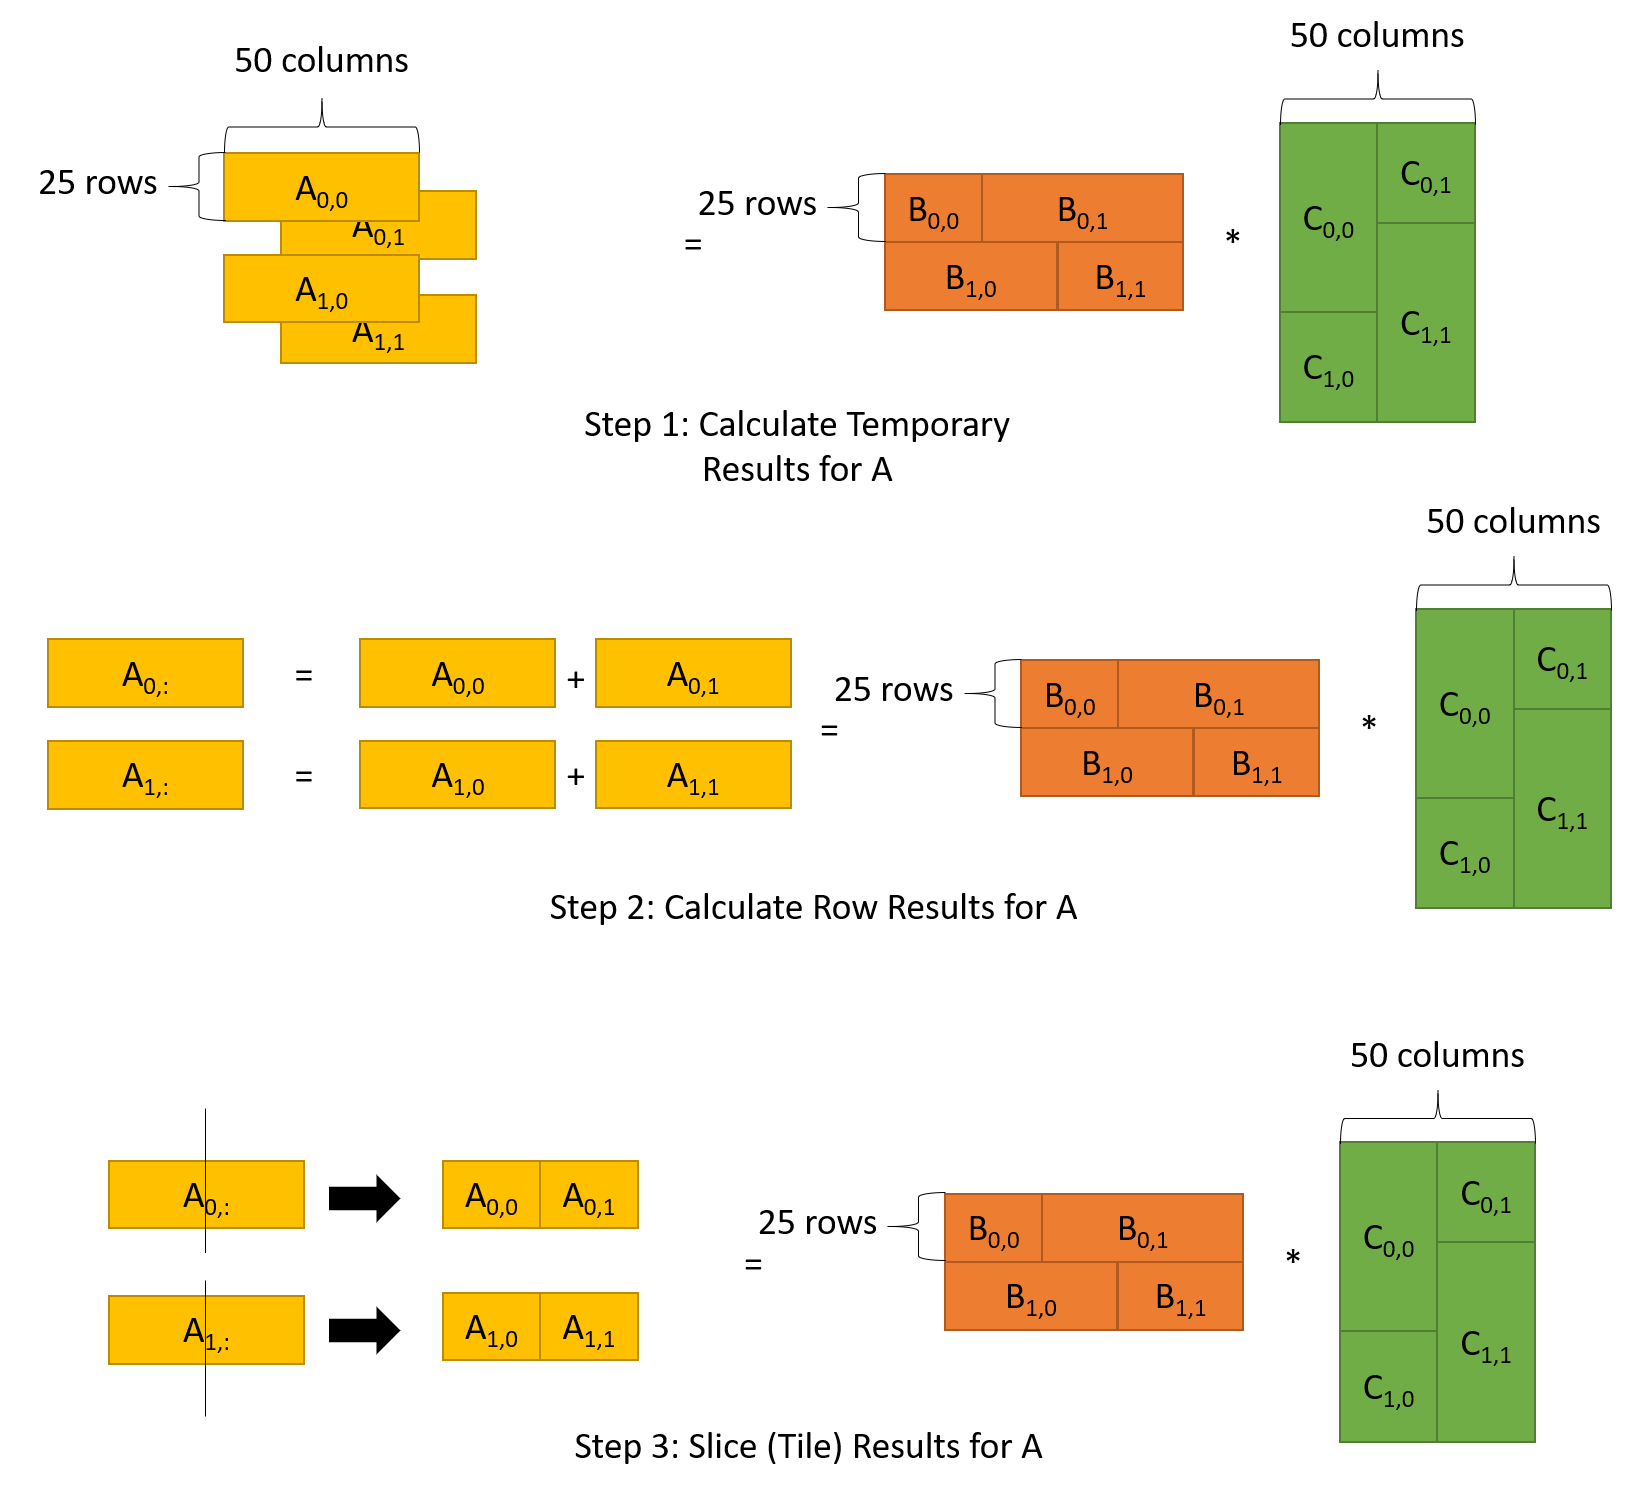
\includegraphics[width=160mm]{intermediate_result_sum}
	\caption{Calculating intermediate sums and tiling them}
	\label{int_sum}
\end{figure}

%%%%%%%%%%%%%%%%%%%%%%%%%%%%%%%%%%%%%%%%%%%%%%%%%%%%%%%%%%%%%%%%%%%%%%%%%%%%%%%%%%%%%%%%%%%

%%%%%%%%%%%%%%%%%%%%%%%%%%%%%%%%%%%%%%%%%%%%%%%%%%%%%%%%%%%%%%%%%%%%%%%%%%%%%%%%%%%%%%%%%%%